%%%%%%%%%%%%%%%%%%%%%%%%%%%%%%%%%%%%%%%%%%%%%%%%%%%%%%%%%%%%%%%%%%%%%%%%%%%%%%%%
%2345678901234567890123456789012345678901234567890123456789012345678901234567890
%        1         2         3         4         5         6         7         8

\documentclass[a4, 10 pt, conference]{ieeeconf}  % Comment this line out
                                                          % if you need a4paper
%\documentclass[a4paper, 10pt, conference]{ieeeconf}      % Use this line for a4
                                                          % paper

\IEEEoverridecommandlockouts                              % This command is only
                                                          % needed if you want to
                                                          % use the \thanks command
\overrideIEEEmargins
% See the \addtolength command later in the file to balance the column lengths
% on the last page of the document



% The following packages can be found on http:\\www.ctan.org
\usepackage{graphicx} % for pdf, bitmapped graphics files
%\usepackage{epsfig} % for postscript graphics files
%\usepackage{mathptmx} % assumes new font selection scheme installed
%\usepackage{times} % assumes new font selection scheme installed
%\usepackage{amsmath} % assumes amsmath package installed
%\usepackage{amssymb}  % assumes amsmath package installed

\title{\LARGE \bf
Learning a `following and chain-building' behavior using PSO
}

%\author{ \parbox{3 in}{\centering Huibert Kwakernaak*
%         \thanks{*Use the $\backslash$thanks command to put information here}\\
%         Faculty of Electrical Engineering, Mathematics and Computer Science\\
%         University of Twente\\
%         7500 AE Enschede, The Netherlands\\
%         {\tt\small h.kwakernaak@autsubmit.com}}
%         \hspace*{ 0.5 in}
%         \parbox{3 in}{ \centering Pradeep Misra**
%         \thanks{**The footnote marks may be inserted manually}\\
%        Department of Electrical Engineering \\
%         Wright State University\\
%         Dayton, OH 45435, USA\\
%         {\tt\small pmisra@cs.wright.edu}}
%}

\author{Alice Concordel$^{1}$, Christoph K\"{o}rner$^{2}$ and Etienne Thalmann$^{3}$% <-this % stops a space
\thanks{This work is a project of the course Distributed intelligent systems by Prof. Alcherio Martinoli}% <-this % stops a space
\thanks{A. Concordel is with Faculty of Mechanical Engineering, School of engineering, Ecole Polytechnique fédérale de Lausanne}
\thanks{C. K\"{o}rner is with the Faculty of Electrical Engineering, Vienna University of Technology} %=============================FILL IN!!!
\thanks{E. Thalmann is with Faculty of Mechanical Engineering, School of engineering, Ecole Polytechnique fédérale de Lausanne}%
}

\begin{document}

\maketitle
\thispagestyle{empty}
\pagestyle{empty}


%%%%%%%%%%%%%%%%%%%%%%%%%%%%%%%%%%%%%%%%%%%%%%%%%%%%%%%%%%%%%%%%%%%%%%%%%%%%%%%%
\begin{abstract}


\end{abstract}


%%%%%%%%%%%%%%%%%%%%%%%%%%%%%%%%%%%%%%%%%%%%%%%%%%%%%%%%%%%%%%%%%%%%%%%%%%%%%%%%
\section{INTRODUCTION}
The goal of this project is to implement a Braitenberg-type controller for movement in formation on e-pucks. For this, a PSO algorithm was implemented, using the weights of the Braitenberg-type controller as a search space. The formation consists of 3 follower robots and one leader that moves with a predefined trajectory. The PSO is run on the Webots platform, which is capable of simulating the behavior of the e-pucks in a realistic way. This makes it possible to run the algorithm and get results much faster than doing it on real e-pucks.

\subsection{Design of PSO}
In order to design a PSO algorithm for a collaborative task, we had to consider three axes: The diversity of the team, the performance evaluation and the solution sharing. We decided  to use a heterogeneous approach with individual performance evaluation and group solution sharing. The idea is to evaluate different solutions on the three followers (heterogenous approach) in order to save computation time and to share the pool of solutions (group solution) to have evolution of the particles. Since we are interested in the performance of each follower with its own particle and not in the performance of the entire chain we need an individual performance evaluation.


\subsection{Design of Fitness Function}
The idea of the fitness function is to evaluate the performance of a controller in being able to follow a leader and stay in chain formation. The design of the fitness function is of primary importance because it defines towards which solution the PSO will converge. Four characteristics were found to be important to evaluate following and chain-building behavior:
\begin{itemize}
\item The range $d$, which is the distance between the follower and the leader, has to be minimized.
\item The relative heading of leader and follower $\Delta \phi $. The heading is defined as the angular orientation of the robot in a fixed frame of reference. The relative heading is zero, when both robots are facing the same way. This angle has to be minimized in order to have nice following. 
\item The bearing $\theta $, which is the angular offset of the leader's position with respect to the heading of the follower. This quantity has to be minimized so that the follower always stays behind the leader.
\item The relative speed between leader and follower $\Delta v $ can be minimized in order to have a smoother following behavior. This was part of our original design but has later been proven unnecessary.
\end{itemize}
The fitness function has to be maximized. We define it as follows:
\begin{equation}\label{fitness}
F=\frac{1}{A*d+B*\theta+C*\Delta \phi+C* \Delta v}
\end{equation}
Where A,B,C,D are coefficients of importance of the different components that are initially set to one and have to be determined.

\section{Methodology}

%\begin{table}
%\caption{An Example of a Table}
%\label{table_example}
%\begin{center}
%\begin{tabular}{|c||c|}
%\hline
%One & Two\\
%\hline
%Three & Four\\
%\hline
%\end{tabular}
%\end{center}
%\end{table}



\addtolength{\textheight}{-3cm}   % This command serves to balance the column lengths
                                  % on the last page of the document manually. It shortens
                                  % the textheight of the last page by a suitable amount.
                                  % This command does not take effect until the next page
                                  % so it should come on the page before the last. Make
                                  % sure that you do not shorten the textheight too much.
                                  
\subsection{Implementation on Webots}

\subsubsection{Environment}
The Webots environment used to simulate the following and chain building consists of one leader e-puck and three followers on a smooth ground free of walls or any obstacles. They followers are initially placed in line behind the leader with a distance of 10 cm between their centres and facing the same way. A supervisor, which is a special kind of robot with more functions, is used to run the PSO algorithm, track the position of the robots, communicate with them and reset their position.

\subsubsection{Supervisor}
The role of the supervisor is to set the initial settings and then to run the PSO. In short, it sends the particles to the followers for their evaluation, gets their fitness back, evolves the swarm and restarts an iteration. After running one full PSO, it uses the best results for the next one and so on until results are satisfying.\\
The number of particles in the swarm is set higher than the number of followers. Since the approach is heterogeneous, the supervisor evaluates them in batches of three by sending one particle (i.e. one set of weights for their Braitenberg controller) to each follower. Then comes the evaluation period during which the followers evaluate the fitness of the controller. To evaluate the fitness of its run according to equation \ref{fitness}, the follower needs to know its coordinates and those of the robot it is following. Thus, while the followers are doing their evaluation run, the supervisor sends to the followers their spatial coordinates (translation and rotation) and those of their respective leader. Once the fitness of each particles is evaluated, it is returned to the supervisor and stored. The supervisor resets the followers and the leader in their initial position and replicates the previous procedure with the following batch of particles. Once all the particles of the swarm have been evaluated, they evolve according to the PSO algorithm using the fitness values obtained for each particle. The new swarm obtained is evaluated  and evolved in the same way as the previous swarm. The number of these evolution iterations is set beforehand.\\
When the last iteration is over, the weights of the particle that returned the best fitness during this run of the PSO are tested by sending them to the followers a chosen number of times and measuring the average fitness of the solution. If the results are better than the previous best, the solution is stored in a text file and set as initial weights for the next PSO run. The entire PSO algorithm is run again like the previous one, each particle being initialized with the best weights so far. This higher level of iterations is run as long as needed to get satisfying results. The weights that had the best fitness evaluation can be extracted from the text file and implemented on the real e-pucks.\\
The supervisor also communicates in a unilateral way with the leader, sending an interruption message every time the positions are reset. The purpose of this is that the leader restarts its trajectory, so as to have always the same trajectory in the case of predefined ones. This was needed at the beginning of the evolutions in order to have all the particles evaluated on a trajectory having the same level of difficulty. This way, weights that are worse than others cannot have a better fitness evaluation just because the trajectory was easier, which would be counter productive.

\subsubsection{Follower}
There are three followers having the same code. The role of a follower is to evaluate the fitness of the particle that is sent by the supervisor. The weights received are used for their Braitenberg-type controller and the fitness is evaluated using \ref{fitness} before being sent back to the supervisor.

\paragraph{Braitenberg-type controller}

\begin{figure}[thpb]
      \centering
      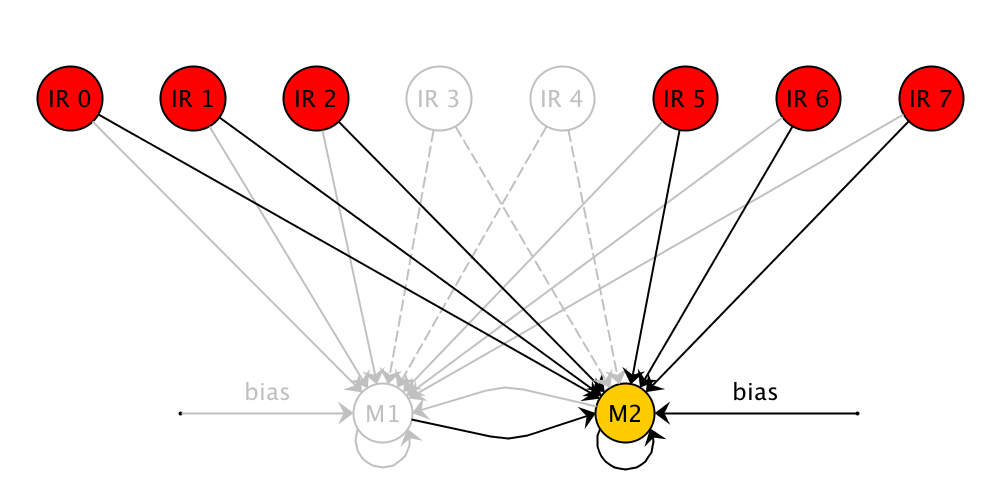
\includegraphics[width = 0.5\textwidth]{images/NNsimplified.png}
      \caption{The simplified neural network (the nodes and links that are greyed are not included on the PSO).}
      \label{fig:nnsimplified}
   \end{figure}

The Braitenberg-type controller is a simple neural network consisting of two neurons corresponding to the wheel motors of the e-puck. As input nodes, the neural network uses the infra-red sensors of the e-puck  and a bias. The outputs are the motor commands of the two wheels. The outputs are also cross-coupled and fed back to their neuron. The complexity of the controller is reduced using symmetry. Indeed, the same weights can be used for the bias, cross-coupling and auto-coupling of both nodes and the weights corresponding to the opposite sensors can be used for the neuron corresponding to the opposite wheel. Moreover, the back sensors can be ignored as they do not play a role in a following behavior. Thus, the number of weights of the controller is reduced to nine: six for the infra-red sensors, one for the bias, one for the cross coupling and one for the auto-coupling.\\
The infra-red sensor values measured in webots were calibrated in order to be close those obtained on the real e-pucks in the chosen lighting conditions. This can be done by updating the lookup tables in webots, which then maps distance to sensor values by linear extrapolation between the inserted data. In order to improve the Braitenberg controller, it was decided to linearise the input by mapping the sensor values back to distance before using them. In order to do this, the inverse function of an exponential regression through the data was used. This improves the quality of the controller because it avoids the exponential increase of the stimulus when the follower gets close to the robot, which makes the response smoother, and it increases the stimulus with distance instead of decreasing it, which makes following easier.\\
The ouput values computed by the Braitenberg controller are transformed into coherent speed values before being sent to the wheels. This is done by mapping the values between -1 and 1 before multiplying them by the maximum speed that the e-pucks can reach. The threshold upon which the speed is set to maximum speed (or minimum speed by taking the negative of the threshold) is set arbitrarily by looking at the range of values returned by the controller.
One last step is done before sending the speed commands to the wheel motors: verifying that the acceleration does not exceed a maximum value. This is done looking at the difference between the new speed and the one of the previous time step. If the difference is larger than the defined maximum acceleration for the e-pucks, the speed corresponding to this maximum value is set.
\paragraph{Fitness evaluation}
Every time a particle is sent to the followers, its fitness has to be evaluated. To do this, webots simulates the behavior of the followers with the given controller and initial chain formation during a certain amount of time steps. The components of the fitness function are evaluated at each time step and averaged at the end. These components are calculated using the position information sent by the supervisor. Each follower calculates at each time step the range, bearing and relative heading between the leader and itself using the received coordinates. At the end of the run, these values are averaged and entered into the fitness function (equation \ref{fitness}). The calculated fitness is sent back to the supervisor and the follower waits until it receives the next particle to start the process again.

\subsubsection{Leader}
The formation performance is strongly dependant on the leader behaviour. It is therefore critical to control this to ensure that the solution obtained is robust. For example, if the leader goes straight forward, then a controller with strong bias and almost no coupling from the sensors will have a good fitness. However, if this controller is then tested with a leader that turns, then the followers will be lost. 

Thus it is important to test the controller on a varied trajectory, containing both left and right turns. A random trajectory will be good for this, but will require a longer evaluation time to ensure that a sufficient variety is obtained. For this reason, the first runs of the PSO (to test its performances and tune its parameters) were run with a predefined trajectory, including a soft turn to the right, then the corresponding turn to the left which brought the robot's heading back to its initial value. The benefit is that all of the parameters acting in the fitness function appear in a short time span, making runs faster. This turned out to be very effective for debugging: the trajectory being the same, the consistency of the fitness values returned was much easier to check. However, this could not be used to evolve the final solution as it would be limited to similar movements of the leader.

So a random, longer trajectory was preferred. At first, random speeds were assigned to the wheels for given time intervals. However, this will give a rather erratic movement. It was optimized such that the new speed of wheel should be 0.4 times the old speed plus 0.6 times a new random speed value (within the wheel command values interval).

Finally, for the testing of the real solution in a small arena, a random movement coupled with obstacle avoidance was loaded onto the leader in order to avoid the robot wandering too far or falling off the test table.

\subsection{PSO characteristics and Optimization}

To get started with the PSO and to examine and understand the behaviour of the robots in Webots and the fitness function we initially started the  noiseless PSO with 10 iterations and 30 fitness steps, to keep the overall simulation time short in the beginning. The leader moved deterministically on a single curve.  Because of this short simulation interval the first optimization results lead to useless controller weights. The only goal in this first step was to examine the quality of the designed fitness function and to test the design of the symmetric controller weights.

To get useful results we extended the number of fitness steps per iteration to 65. The trajectory of the leader was still deterministic, but it consisted of two opposite curves and a straight part in between. The velocity of the leader was constant. After evolving the PSO several times with random initial particles and velocities we observed a big variance in the quality of the results. So we tried to improve the quality of the PSO with implementing bounded constraints for the PSO \cite{c1}. With initially starting an iteration of the optimization with the last best solution we could achieve better results in less number of iterations compared to random initialization of particles. Increasing the number of PSO iterations to 40 extended the overall optimization time, but lead to useful results after each optimization. After the implementation of a function, that stored the best controller weights to a file, if they were better than the previous best, we could run the optimization with good initial particles in an infinite loop over the night. Applying the optimization results to the followers in Webots, the robots could follow the leader perfectly under the given (optimal) constraints.

In the next step we extended the follower model to have a more realistic behaviour. Therefore we added noisy nonlinear sensor values for the proximity sensors of the epucks. We configured the PSO for a noisy system, which re-evaluates the best performance of an PSO iteration an doubles the number of iterations per optimization step. We also complicated the leaders behaviour, such that the trajectory is random and 180 simulation steps long. We seeded the random number generator with the actual time stamp to get different random values for each optimization but with giving up reproducibility of the solutions. For the overnight simulation we started one PSO with good initial particles and random velocities and another with random particles and random velocities. The performance for the optimization with initial particles was twice as good as the one with initial random particles.



swarmsize, neigborhoods
optiomize the fitness etc noise resistant
no penalty fo rmax speed etc
bearing more important... ABCD

%%%%%%%%%%%%%%%%%%%%%%%%%%%%%%%%%%%%%%%%%%%%%%%%%%%%%%%%%%%%%%%%%%%%%%%%%%%%%%%%
\section{Results}
trajectories and iterations
%%%%%%%%%%%%%%%%%%%%%%%%%%%%%%%%%%%%%%%%%%%%%%%%%%%%%%%%%%%%%%%%%
\section{Conclusions}

%%%%%%%%%%%%%%%%%%%%%%%%%%%%%%%%%%%%%%%%%%%%%%%%%%%%%%%%%%%%%%%%%%%%%%%%%%%%%%%%
\section{ACKNOWLEDGMENTS}
The authors would like to thank Alcherio Martinoli for an exciting and challenging course. Special thanks also to Milos Vasic, for his precious advice and support, as well as all the other teaching assistants of the course for their work throughout the semester.

\begin{thebibliography}{99}

\bibitem{c1}
E.F. Campana, M. Diez, G. Fasano and D. Peri, "Initial Particles Position for PSO,
in Bound Constrained Optimization" in Advances in Swarm Intelligence, {\it 4th International Conference, ICSI 2013; Harbin, China, June 2013; Proceedings, Part I}, Springer-Verlag Berlin Heidelberg, 2013, pp 112-119.

\end{thebibliography}

\end{document}
